\documentclass{article}

\usepackage[dvips]{graphics}

\title{Title of the Paper}
\author{Bob Smith}

% Set properties of paper
\setlength{\textheight}{8.75in}
\setlength{\textwidth}{6.8in}
\setlength{\topmargin}{0.25in}
\setlength{\headheight}{0.0in}
\setlength{\headsep}{0.0in}
\setlength{\oddsidemargin}{-.19in}
\setlength{\parindent}{1pc}

% Here's how to create macros
\newcommand{\summation}[3]{\sum^{#2}_{#1} #3}
\newcommand{\cond}[5]{#1 = \left\{ \begin{array}{ll}
                                        #2 & \mbox{#3} \\
                                        #4 & \mbox{#5}
                                     \end{array}
                                \right.}

\begin{document}

\maketitle

\begin{abstract}
This abstract is very abstract
\end{abstract}

\setcounter{page}{1}

\chapter{Introduction}
\label{chap:intro}

Today people use computers to make phone calls, watch TV, send
instant messages to their friends, play games with other people,
and buy most anything you can think of---from songs to automobiles.  The
ability for programs to communicate over the Internet makes all this
possible.  It's hard to say how many individual computers are now
reachable over the Internet, but we can safely say that it is growing
rapidly; it won't be long before the number is in the billions.
Moreover, new applications are being developed every day.  With the
push for ever increasing bandwidth and access, the impact of the
Internet will continue to grow for the forseeable future.

How \emph{does\/} a program communicate with another program over a
network?  The goal of this book is to \emph{start\/} you on the road
to understanding the answer to that question, in the context of the
C programming language.  For a long time, C was the language of choice
for implementing network communication softward.  Indeed, the 
application programming interface (API) known as \defn{sockets} was
first developed in C.

Before we delve into the details of sockets, however, it is worth
taking a brief look at the big picture of networks and protocols to
see where our code will fit in.  Our goal here is \emph{not\/} to
teach you how networks and TCP/IP work---many fine texts are available
for that purpose~\cite{ComerV1,ComerV3,PandD,StevensV1,StevensV2}---but
rather to introduce some basic concepts and terminology.

\section{Networks, Packets, and Protocols}

A computer network consists of machines interconnected by
communication channels. We call these machines \emph{hosts} and
\emph{routers}.  Hosts are computers that run applications such as
your Web browser, your IM agent, or a file-sharing program.
The application programs running on hosts are the
real ``users'' of the network.  Routers (also called \emph{gateways}) are machines whose job is to
relay, or \emph{forward}, information from one communication channel
to another.  They may run programs but typically do not run
application programs.  For our purposes, a \emph{communication
channel} is a means of conveying sequences of bytes from one host to
another; it may be a wired (e.g., Ethernet), a wireless (e.g., WiFi), or
other connection.

Routers are important simply because it is not practical to connect
every host directly to every other host. Instead, a few hosts connect
to a router, which connects to other routers, and so on to form the
network.  This arrangement lets each machine get by with a relatively
small number of communication channels; most hosts need only one.
Programs that exchange information over the network, however, do not
interact directly with routers and generally remain blissfully unaware
of their existence.

By \emph{information} we mean sequences of {bytes} that are
constructed and interpreted by programs. In the context of computer
networks, these byte sequences are generally called \emph{packets}.  A
packet contains control information that the network uses to do its
job and sometimes also includes user data.  An example is information
identifying the packet's destination. Routers use such control
information to figure out how to forward each packet.

A \emph{protocol} is an agreement about the packets exchanged by
communicating programs and what they mean.  A protocol tells how
packets are structured---for example, where the destination
information is located in the packet and how big it is---as well as
how the information is to be interpreted.  A protocol is usually
designed to solve a specific problem using given capabilities.  For
example, the \emph{HyperText Transfer Protocol (HTTP)} solves the
problem of transferring hypertext objects between servers, where they
are stored or generated,
and Web browsers that make them visible and useful to users.
Instant messaging protocols solve the problem of enabling two or more
users to exchange brief text messages.

Implementing a useful network requires solving a large number of
different problems. To keep things manageable and modular,
different protocols are designed to solve different sets of problems.
TCP/IP is one such collection of solutions, sometimes called a
\emph{protocol suite}.  It happens to be the suite of protocols used
in the Internet, but it can be used in stand-alone private networks as
well.  Henceforth when we talk about the \emph{network}, we mean any
network that uses the TCP/IP protocol suite.  The main protocols in
the TCP/IP suite are the Internet Protocol (IP), the Transmission
Control Protocol (TCP), and the User Datagram Protocol (UDP).

It turns out to be useful to organize protocols into \emph{layers};
TCP/IP and virtually all other protocol suites are organized this way.
Figure~\ref{fig:IPnet} shows the relationships among the protocols,
applications, and the sockets API in the hosts and routers, as well as
the flow of data from one application (using TCP) to another.  The
boxes labeled TCP, UDP, and IP represent implementations of those
protocols. Such implementations typically reside in the operating
system of a host.  Applications access the services provided by UDP
and TCP through the sockets API, represented as a dashed line.  The arrow 
depicts the flow of data
from the application, through the TCP and IP implementations, through
the network, and back up through the IP and TCP implementations at the
other end.

\begin{figure}[htbp]
\jfigs{figures/IPnet.eps}{\textwidth}
\caption{\label{fig:IPnet}A TCP/IP Network}
\end{figure}

In TCP/IP, the bottom layer consists of the underlying communication
channels---for example, Ethernet or dial-up modem connections.  Those
channels are used by the \emph{network layer}, which deals with the
problem of forwarding packets toward their destination (i.e., what
routers do).  The single network layer protocol in the TCP/IP suite is
the Internet Protocol; it solves the problem of making the sequence of
channels and routers between any two hosts look like a single
host-to-host channel.

The Internet Protocol provides a \emph{datagram} service: every packet
is handled and delivered by the network independently, like letters or
parcels sent via the postal system.  To make this work, each IP packet
has to contain the \emph{address} of its destination, just as every
package that you mail is addressed to somebody.  (We'll say more about
addresses shortly.)  Although most delivery companies guarantee
delivery of a package, IP is only a best-effort protocol: it attempts
to deliver each packet, but it can (and occasionally does) lose,
reorder, or duplicate packets in transit through the network.

The layer above IP is called the \emph{transport layer}.  It offers a
choice between two protocols: TCP and UDP.  Each builds on the service
provided by IP, but they do so in different ways to provide different
kinds of transport, which are used by \emph{application protocols}
with different needs.  TCP and UDP have one function in common:
addressing.  Recall that IP delivers packets to hosts; clearly, a
finer granularity of addressing is needed to get a packet to a
particular application program, perhaps one of many using the network on the
same host.  Both TCP and UDP use addresses, called \emph{port
numbers}, to identify applications within hosts.  TCP and UDP are called
\emph{end-to-end transport protocols} because they carry data all the
way from one program to another (whereas IP only carries data from one
host to another).

TCP is designed to detect and recover from the losses, duplications,
and other errors that may occur in the host-to-host channel provided
by IP.  TCP provides a \emph{reliable byte-stream} channel, so that
applications do not have to deal with these problems.  It is a
\emph{connection-oriented} protocol: before using it to communicate,
two programs must first {establish a TCP connection}, which involves
completing an exchange of \emph{handshake messages} between the TCP
implementations on the two communicating computers.  Using TCP is also
similar in many ways to file input/output (I/O). In fact, a file that
is written by one program and read by another is a reasonable model of
communication over a TCP connection.  UDP, on the other hand, does not
attempt to recover from errors experienced by IP; it simply extends
the IP best-effort datagram service so that it works between
application programs instead of between hosts.  Thus, applications
that use UDP must be prepared to deal with losses, reordering, and
so~on.

\section{About Addresses}
\label{sect:introaddr}

When you mail a letter, you provide the address of the recipient in a
form that the postal service can understand. Before you can talk to
someone on the phone, you must supply a phone number to the telephone
system.  In a similar way, before a program can communicate with
another program, it must tell the network something to identify the other
program.  In TCP/IP, it takes two pieces of information to identify a
particular program: an \emph{Internet address}, used by IP, and a
\emph{port number}, the additional address interpreted by the
transport protocol (TCP or UDP).

Internet addresses are binary numbers.  They come in two flavors,
corresponding to the two versions of the Internet Protocol that have
been standardized.  The most common is version~4
(``IPv4'',~\cite{RFC791}); the other is 
version~6 (``IPv6'',~\cite{RFC2460}), which is just beginning to be
deployed.  IPv4 addresses are 32 bits long; because this is only
enough to identify about 4 billion distinct destinations, they are not
really big enough for today's Internet.   (That may seem like a lot,
but because of the way they are allocated, many are wasted.  More than
half of the total IPv4 address space has already been allocated.)
For that reason, IPv6 was introduced.  IPv6 addresses are 128 bits long.

\subsection{Writing Down IP Addresses}

In representing Internet addresses for human consumption (as opposed to
using them inside programs), different conventions are used for the two
versions of IP.  IPv4 addresses are conventionally written as a group of
four decimal numbers separated by periods (e.g., 10.1.2.3); this is
called the \defn{dotted-quad} notation.  The four numbers in a
dotted-quad string represent the contents of the four bytes of the
Internet address---thus, each is a number between 0 and 255.

The sixteen bytes of an IPv6 address, on the other hand,
by convention are represented as groups of hexadecimal digits, separated by
colons (e.g., 2000:fdb8:0000:0000:0001:00ab:853c:39a1).  Each group of
digits represents two bytes of the address; leading zeros may be
omitted, so the fifth and sixth groups
in the foregoing example might be rendered as just :1:ab:.
Also, consecutive groups that contain only zeros may be omitted
altogether (while leaving the colons that would separate them from the
rest of the address).  So the example above could be written as
2000:fdb8::1:00ab:853c:39a1.

Technically, each Internet address refers to the connection between a
host and an underlying communication channel---in other words, a
\emph{network interface}.  A host may have several interfaces; it is
not uncommon, for example, for a host to have connections to both
wired (Ethernet) and wireless (WiFi) networks.
Because each such network connection belongs to a
single host, an Internet address identifies a host as well as its
connection to the network.  However, the converse is not true, because
a single host can have multiple interfaces, and each interface can
have multiple addresses.  (In fact, the same interface can have both IPv4
and IPv6 addresses.)

%%%%%%%% NEW STUFF
\subsection{Dealing with Two Versions}

When the first edition of this book was written, IPv6 was not widely
supported.  Today most systems are capable of supporting IPv6 ``out of the box.''
To smooth the transition from IPv4 to IPv6, most systems are \defn{dual-stack\/},
simultaneously supporting both IPv4 and IPv6.  In such systems, each
network interface (channel connection) may have at least one IPv4 address
and one IPv6 address.  

The existence of two versions of IP complicates life for the socket
programmer.  In general, you will need to choose either
IPv4 or IPv6 as the underlying protocol when you create a socket to
communicate.  So how can you write an application that works with both versions?
Fortunately, dual-stack systems handle interoperability by supporting both
protocol versions and allowing IPv6 applications
to communication with either IPv4 or IPv6 applications.  Of course, IPv4 and IPv6 addresses
are quite different; however, IPv4 addresses can be mapped into IPv6 addresses using
\defn{IPv4 mapped addresses}.  An IPv4 mapped
address is formed by prefixing the four bytes in the IPv4 address with ::fff.  For
example, the IPv4 mapped address for 132.3.23.7 is ::ffff:132.3.23.7.  To aid
in human readability, the last four
bytes are typically written in dotted-quad notation.  We discuss protocol interoperability
in greater detail in Chapter~\ref{chap:addrindep}.

%As \Fig{dualstack} shows, once you make that choice, 
%information sent through the socket will stay within the corresponding
%side of the stack from end-to-end.

%\begin{figure}[tbp]
%\jfigs{figures/dualstack2.eps}{\textwidth}
%\caption{System with both IPv4 and IPv6 support.\label{dualstack}}
%\end{figure}

%
Unfortunately, having an IPv6 Internet address
is \emph{not\/} sufficient to enable you to communicate with every
other IPv6-enabled host across the Internet.  To do that, you must also
arrange with your Internet Service Provider to provide IPv6 forwarding
service.

\subsection{Port Numbers}

We mentioned earlier that it takes \emph{two\/} pieces of address to
get a message to a program.
The \emph{port number\/} in TCP or UDP is always interpreted relative to an
Internet address.
Returning to our earlier analogies, a port number
corresponds to a room number at a given street address, say, that of a
large building.  The postal service uses the street address to get the
letter to a mailbox; whoever empties the mailbox is then responsible
for getting the letter to the proper room within the building. Or
consider a company with an internal telephone system: to speak to an
individual in the company, you first dial the company's main phone
number to connect to the internal telephone system and then dial the
extension of the particular telephone of the individual that you wish
to speak with.  In these analogies, the Internet address is the street
address or the company's main number, whereas the port corresponds to
the room number or telephone extension.  Port numbers are the same in
both IPv4 and IPv6: 16-bit
unsigned binary numbers. Thus, each one is in the range 1 to 65,535 (0 is
reserved).

\subsection{Special Addresses}

In each version of IP, certain special-purpose addresses are defined.
One of these that is worth knowing is the \emph{loopback address},
which is always assigned to a special \defn{loopback
interface}, a virtual device
that simply echoes transmitted packets right back to the
sender.  The loopback interface is very useful for testing, because
packets sent to that address are immediately returned back to the
destination.  Moreover, it is present on every host, and can be
used even when a computer has no other interfaces (i.e.,
is not connected to the network).
The loopback address for IPv4 is 127.0.0.1;\footnote{Technically
any IPv4 address beginning with 127 should loop back.}
for IPv6 it is 0:0:0:0:0:0:0:1 (or just ::1).

Another group of IPv4 addresses reserved for a special purpose
includes those reserved for ``private use''.
This group includes all IPv4 addresses that start with
10 or 192.168, as well as those whose first number is 172 and whose
second number is between 16 and 31.  (There is no corresponding class
for IPv6.)
These addresses were originally designated for use in private networks
that are \emph{not\/} part of the global Internet.
Today they are often used in homes and small offices that are connected 
to the Internet through a \emph{network address translation\/} (NAT)\cite{RFC3022}
device.  Such a device acts like a router that
translates (rewrites) the addresses and ports
in packets as it forwards them.  More precisely, it maps
(private address, port) pairs in packets on one of its interfaces
to (public address, port) pairs on the other interface.
This enables a small group of hosts (e.g., those on a home network) to
effectively ``share'' a single IP address.
The importance of these addresses is that \emph{they cannot be reached
from the global Internet}.  If you are trying out the code in
this book on a machine that has an address in the private-use class
(e.g., on your home network),
and you are trying to communicate with another host that does
\emph{not\/} have one of these addresses, in general you will not
succeed unless the host with the private address initiates
communication---and even then you may fail.

A related class contains the \emph{link-local}, or
 ``autoconfiguration'' addresses.  For IPv4, such addresses
begin with 169.254.  For  IPv6, any address whose first 16-bit chunk is
FE80, FE90, FEA0, or FEB0 is a link-local address.
This addresses can \emph{only\/} be used for communication between
hosts connected to the same network; routers will not forward packets
that have such addresses as their destination.

Finally, another class consists of \emph{multicast}
addresses.  Whereas regular IP (sometimes called
``unicast'') addresses refer to a single destination, multicast
addresses potentially refer to an arbitrary number of destinations.
%
Multicasting is an advanced subject that we cover briefly in
Chapter~\ref{chap:advanced}.  In IPv4, multicast addresses in
dotted-quad format have a first number in the range 224 to 239.
In IPv6, multicast addresses start with FF.

\section{About Names}

Most likely you are accustomed to referring to hosts by \emph{name}
(e.g., host.example.com).  However, the Internet protocols deal with
addresses (binary numbers), not names.  You should understand that the use of
names instead of addresses is a convenience feature that is
independent of the basic service provided by TCP/IP---you can write
and use TCP/IP applications without ever using a name.  When you use a
name to identify a communication endpoint, the system  does some
extra work to \emph{resolve} the name into an address.
%
This extra step is often worth it, for a couple of reasons. First,
names are obviously easier for humans to remember than dotted-quads
(or, in the case of IPv6,  strings of hexadecimal digits).
Second, names provide a level of indirection, which insulates users
from IP address changes.  During the writing of the first edition of
this book, the address of the Web server \emph{www.mkp.com}\/
changed.
%
Because we always refer to that Web server by name,
\emph{www.mkp.com} resolves to the current Internet address instead
of 208.164.121.48.  The change in IP address is transparent to programs that use the
name to access the Web server.

The name-resolution service can access information from a wide variety
of sources.  Two of the primary sources are the \defn{Domain Name
System (DNS)} and local configuration databases.  The
DNS~\cite{RFC1034} is a distributed database that maps \emph{domain
names} such as \emph{www.mkp.com} to Internet addresses and other
information; the DNS protocol~\cite{RFC1035} allows hosts connected
to the Internet to retrieve information from that database using TCP
or UDP.  Local configuration databases are generally OS-specific
mechanisms for local name-to-Internet address mappings.

\section{Clients and Servers}

In our postal and telephone analogies, each communication
is initiated by one party, who sends a letter or makes the telephone
call, while the other party responds to the initiator's contact by
sending a return letter or picking up the phone and talking.  Internet
communication is similar.  The terms \defn{client} and \defn{server}
refer to these roles: The client program initiates communication,
while the server program waits passively for and then responds to
clients that contact it.  Together, the client and server compose the
\emph{application}.  The terms \emph{client} and \emph{server} are
descriptive of the typical situation in which the server makes a
particular capability---for example, a database service---available to
any client that is able to communicate with~it.

Whether a program is acting as a client or server determines the
general form of its use of the sockets API to establish communication
with its \defn{peer}.  (The client is the peer of the server and vice
versa.)  Beyond that, the client-server distinction is important
because {the client needs to know the server's address and port
initially}, but not vice versa.  With the sockets API, the server can,
if necessary, learn the client's address information when it receives
the initial communication from the client.  This is analogous to a
telephone call---in order to be called, a person does not need to know
the telephone number of the caller.  As with a telephone call, once
the connection is established, the distinction between server and
client disappears.

How does a client find out a server's IP address and port number?
Usually, the client knows the name of the server it wants---for
example, from a \emph{Universal Resource Locator (URL)} such as
\emph{http://www.mkp.com}---and uses the name-resolution service to
learn the corresponding Internet address.

Finding a server's port number is a different story.  In principle,
servers can use any port, but the client must be able to learn what it
is.  In the Internet, there is a convention of assigning {well-known
port numbers} to certain applications. The Internet Assigned Number
Authority (IANA) oversees this assignment.  For example, port number
80 has been assigned to the \emph{Hypertext Transfer Protocol}
\emph{(HTTP)}.  When you run an HTTP client browser, it tries to
contact the web server on that port by default. A list of all the
assigned port numbers is maintained by the numbering authority of the
Internet (see \emph{http://www.iana.org/assignments/port-numbers}).

Many of you have heard of an alternative to client-server called peer-to-peer
(P2P).  In P2P, applications both consume and provide service,
unlike the traditional client-server architecture where
servers provide service
and clients consume.  In fact, P2P nodes are sometimes called ``servents,'' combining
the words server and client.  So do you need to learn a different set of technologies to
program for P2P instead of client-server?  No.  In Sockets, client vs. server
merely distinguishes who makes the initial connection and who wait for connections.
P2P applications typically both initiate connections (to existing P2P nodes)
and accept connections (from other P2P nodes).  After reading this book, you'll
be able to write P2P applications just as well as client-server.

\section{What Is a Socket?}

A \emph{socket} is an abstraction through which an application may
send and receive data, in much the same way as an open file handle
allows an application to read and write data to stable storage.  A
socket allows an application to plug in to the network and communicate
with other applications that are plugged in to the same
network. Information written to the socket by an application on one
machine can be read by an application on a different machine and vice
versa.

Different types of sockets correspond to different underlying protocol
suites and different stacks of protocols within a suite.  This book
deals only with the TCP/IP protocol suite.  The main types of sockets
in TCP/IP today are \emph{stream sockets} and \emph{datagram sockets}.
Stream sockets use TCP as the end-to-end protocol (with IP underneath)
and thus provide a reliable byte-stream service.  A TCP/IP stream
socket represents one end of a TCP connection.  Datagram sockets use
UDP (again, with IP underneath) and thus provide a best-effort
datagram service that applications can use to send individual messages
up to about 65,500 bytes in length.  Stream and datagram sockets are
also supported by other protocol suites, but
 this book deals only with TCP stream sockets and UDP datagram
sockets.  A TCP/IP socket is uniquely identified by an Internet
address, an end-to-end protocol (TCP or UDP), and a port number.  As
you proceed, you will encounter several ways for a socket to become
bound to an address.

Figure~\ref{fig:sockstack} depicts the logical relationships among
applications, socket abstractions, protocols, and port numbers within
a single host.  There are several things to note about these
relationships.  First, a program can have multiple sockets in use
at the same time.  It is also that multiple programs can be using the
same socket abstraction at the same time, although this is less common.
The figure shows that each socket has an associated local TCP or UDP port,
which is used to direct incoming packets to the application that is
supposed to receive them.
Earlier we said that a port identifies an application on a host.
Actually, a port identifies a socket on a host.  
There is more to it than this, however,
because as Figure~\ref{fig:sockstack} shows, more than one socket can
be associated with one local port.  This is most common with TCP
sockets; fortunately, you need not understand the details to write
client-server programs that use TCP sockets.  The full story will be
revealed in Chapter~\ref{chap:under}.


\begin{figure}[htbp]
%\jfigs{figures/ja01f02.eps}{}
% XXXX what macro?
\jfigs{figures/sockstack.eps}{0.5\textwidth}
\caption{Sockets, protocols, and ports.\label{fig:sockstack}}
\end{figure}

\begin{exercises}

\item Report your IP addresses using the \texttt{ifconfig} command in *NIX or 
the \texttt{ipconfig} command in Windows.  Identify the addresses that are
IPv6.

\item Report the name of the on which you are working by using the 
\texttt{hostname} command.

\item Can you find the IP address of any of your directly-connected routers?

\item Use Internet search to try and discover what happened to IPv5?

\item Write the following IPv6 address using as few characters as possible:
2345:0000:0000:A432:0000:0000:0000:0023

\item Can you think of a real-life example of communication that does
not fit the client-server model?

\item To how many different kinds of networks is your home connected?
How many support two-way transport?

\item IP is a best-effort protocol, requiring that information
be broken down into datagrams, which may be lost, duplicated, or
reordered.  TCP hides all of this, providing a reliable service that
takes and delivers an unbroken stream of bytes.  How might you go
about providing TCP service on top of IP?  Why would anybody use UDP
when TCP is available?

\end{exercises}

\section{Meat of the paper}

Here's the meat of the paper.

Figure~\ref{fig:picture} has a picture.

\begin{figure}[htbp]
\centerline{\resizebox{5in}{!}{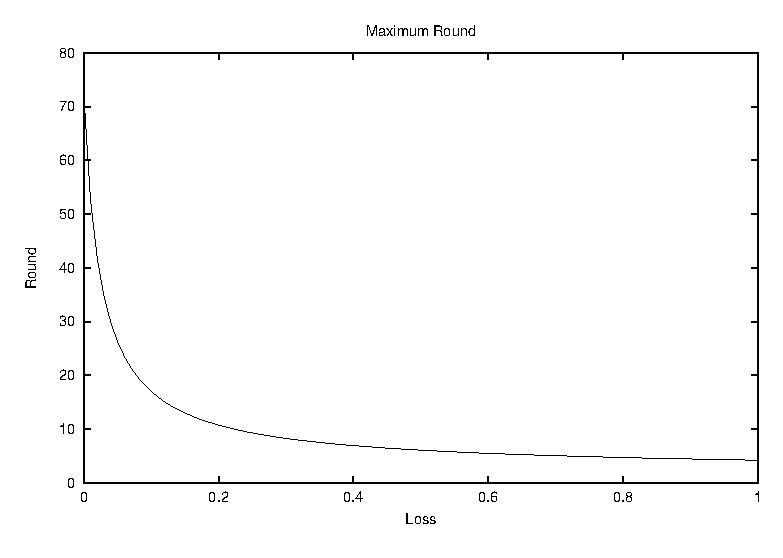
\includegraphics{maxround.ps}}}
\caption{\label{fig:picture} Picture of something that relates to Table~\ref{tab:mytable}}
\end{figure}

\noindent Here's the same picture but in another spot.
\begin{figure}[htbp]
\centerline{\resizebox{5in}{!}{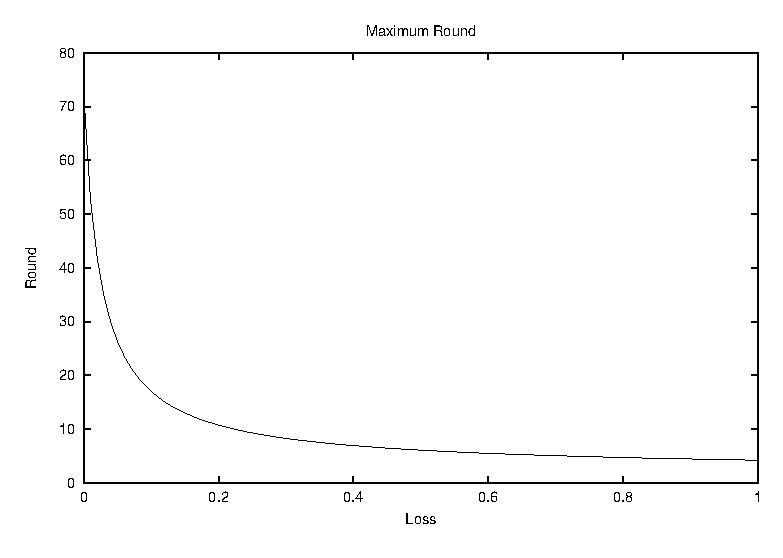
\includegraphics{maxround.ps}}}
\caption{\label{fig:repeatpicture} Repeat of Figure~\ref{fig:picture}}
\end{figure}

Here we use the macros

\[\summation{i=0}{N}{X^i}\]

\[\cond{X}{5}{if sky is blue}{6}{otherwise}\]

\section{Conclusions}

\bibliography{bib}
\bibliographystyle{apalike}

\end{document}
